\chapter{Protein Classification}
\label{ch:classification}

By the mid-1990s the Protein Data Bank held roughly ten thousand structures, and
the number was climbing fast. Christine Orengo and Janet Thornton, working at
University College London, faced a problem that was equal parts intellectual and
logistical: how should one organize this growing collection~\cite{orengo1997}? Proteins plainly fell
into families. Globins resembled other globins; immunoglobulin domains looked like
other immunoglobulin domains. But the boundaries between families were blurry, the
criteria for grouping were subjective, and two experts asked to sort the same set
of structures often disagreed on where to draw the lines.\sidenote{Alexei Murzin,
working independently at the MRC Laboratory of Molecular Biology in Cambridge, was
confronting the same question and would publish SCOP the same year Orengo
published CATH.}

The difficulty was not merely taxonomic. The same fold appeared again and again in
proteins with no detectable sequence similarity. The TIM barrel, an
eight-stranded $(\beta/\alpha)_8$ cylinder, showed up in triosephosphate
isomerase, in glycolate oxidase, in tryptophan synthase, in ribulose-phosphate
epimerase. These proteins catalyze unrelated reactions on unrelated substrates.
Either they diverged from a common ancestor so long ago that every trace of
sequence relationship has been erased, or evolution independently arrived at the
same structural solution multiple times. Both possibilities are plausible, and
distinguishing between them remains one of the harder problems in molecular
evolution. Classification had to accommodate this ambiguity without pretending to
resolve it.

This chapter treats two interleaved questions. First, what hierarchies have been
proposed for organizing protein structures, and what principles guide them? Second,
how does one measure structural similarity in the first place, so that the
classification can rest on quantitative ground rather than visual impression alone?


\section{The SCOP hierarchy}
\label{sec:scop}

\newthought{Alexei Murzin and colleagues} published the Structural Classification
of Proteins (SCOP) database in 1995~\cite{murzin1995}. Its organizing principle was evolutionary:
structures belong together when they share a common ancestor. The classification is
a strict hierarchy with four levels.

At the top sit the \emph{classes}, defined by secondary-structure composition.
``All-$\alpha$'' proteins are built predominantly from $\alpha$-helices;
``all-$\beta$'' proteins from $\beta$-sheets; ``$\alpha/\beta$'' proteins
alternate $\alpha$-helices and $\beta$-strands along the sequence, typically
producing parallel $\beta$-sheets flanked by helices; and ``$\alpha+\beta$''
proteins contain both types of secondary structure in segregated regions rather
than alternating them.\sidenote{SCOP also includes smaller classes for
multi-domain proteins, membrane and cell-surface proteins, and small proteins
stabilized mainly by disulfides or metal ions.} Class assignment is the coarsest
cut and often unambiguous, though borderline cases between $\alpha/\beta$ and
$\alpha+\beta$ require judgment.

Below class lies the \emph{fold} level. Two proteins share a fold if their major
secondary-structure elements are arranged with the same topology and spatial
relationships. The Rossmann fold, for instance, groups all proteins containing a
parallel $\beta$-sheet of at least three strands connected by $\alpha$-helices
such that the strand order in the sheet is 321456. A shared fold does not imply
shared ancestry; it may reflect physical constraints on how secondary structures
pack, or convergent evolution toward a thermodynamically favorable architecture.

The \emph{superfamily} level collects proteins that probably derive from a common
ancestor but have diverged so far that sequence comparison alone cannot establish
the relationship. The evidence is structural: similar folds combined with similar
functional features or scattered sequence motifs at catalytic sites. Assignment at
this level is an evolutionary hypothesis, not a proven fact.

Finally, the \emph{family} level groups proteins with clear evolutionary
relationships visible in sequence alignments, typically above 30\% identity or
with statistically significant sequence similarity detected by tools such as
PSI-BLAST.

SCOP was manually curated. Murzin and a small team inspected each new structure,
decided where it belonged, and placed it in the hierarchy. This manual approach
had strengths: expert knowledge could resolve ambiguities that automated methods
would handle clumsily. It also had an obvious weakness. As the PDB grew from ten
thousand structures to over two hundred thousand, manual curation could not keep
pace. SCOP2, a later revision, introduced a graph-based representation that
relaxed the strict tree hierarchy, allowing proteins to participate in multiple
relationships simultaneously~\cite{andreeva2014}. But the curation bottleneck persisted.


\section{The CATH hierarchy}
\label{sec:cath}

\newthought{Orengo and Thornton's} CATH database~\cite{orengo1997}, published in
1997, took a different approach. Where SCOP relied almost entirely on expert
judgment, CATH mixed automated structure-comparison algorithms with manual
oversight. The name encodes its four-level hierarchy: Class, Architecture,
Topology, and Homologous superfamily.

\emph{Class} in CATH, as in SCOP, is determined by secondary-structure content.
The three main classes are ``mainly alpha,'' ``mainly beta,'' and ``mixed alpha
and beta.'' Assignment uses the fraction of residues in $\alpha$-helices versus
$\beta$-strands, computed automatically from atomic coordinates using DSSP~\cite{kabsch1983} or
similar secondary-structure assignment programs.

\emph{Architecture} describes the gross spatial arrangement of secondary-structure
elements, ignoring their connectivity. A four-helix bundle has a different
architecture from a barrel or a sandwich. Architecture is assigned by a
combination of automated comparison and visual inspection. This level has no
direct analogue in SCOP; it captures shape without committing to a topological
definition.\sidenote{The architecture level was partly inspired by the observation
that proteins with different topologies can share the same overall shape. A
$\beta$-sandwich, for instance, can be built with many different strand
connectivities.}

\emph{Topology}, equivalent to fold in SCOP, considers both the arrangement and
the connectivity of secondary-structure elements. Proteins share a topology if
they can be superimposed with consistent chain direction through matched secondary
structures. The structure comparison algorithm SSAP (Sequential Structure
Alignment Program) was central to topology assignment: protein pairs scoring above
a threshold in SSAP were grouped together~\cite{taylor1990}.

\emph{Homologous superfamily}, the deepest level, groups proteins that share a
common evolutionary origin. Evidence comes from sequence similarity, structural
similarity, and functional similarity considered jointly. The criteria are
stringent: high SSAP scores combined with either sequence identity above 35\% or
convincing HMM-based detection of remote homology.

\begin{figure*}
  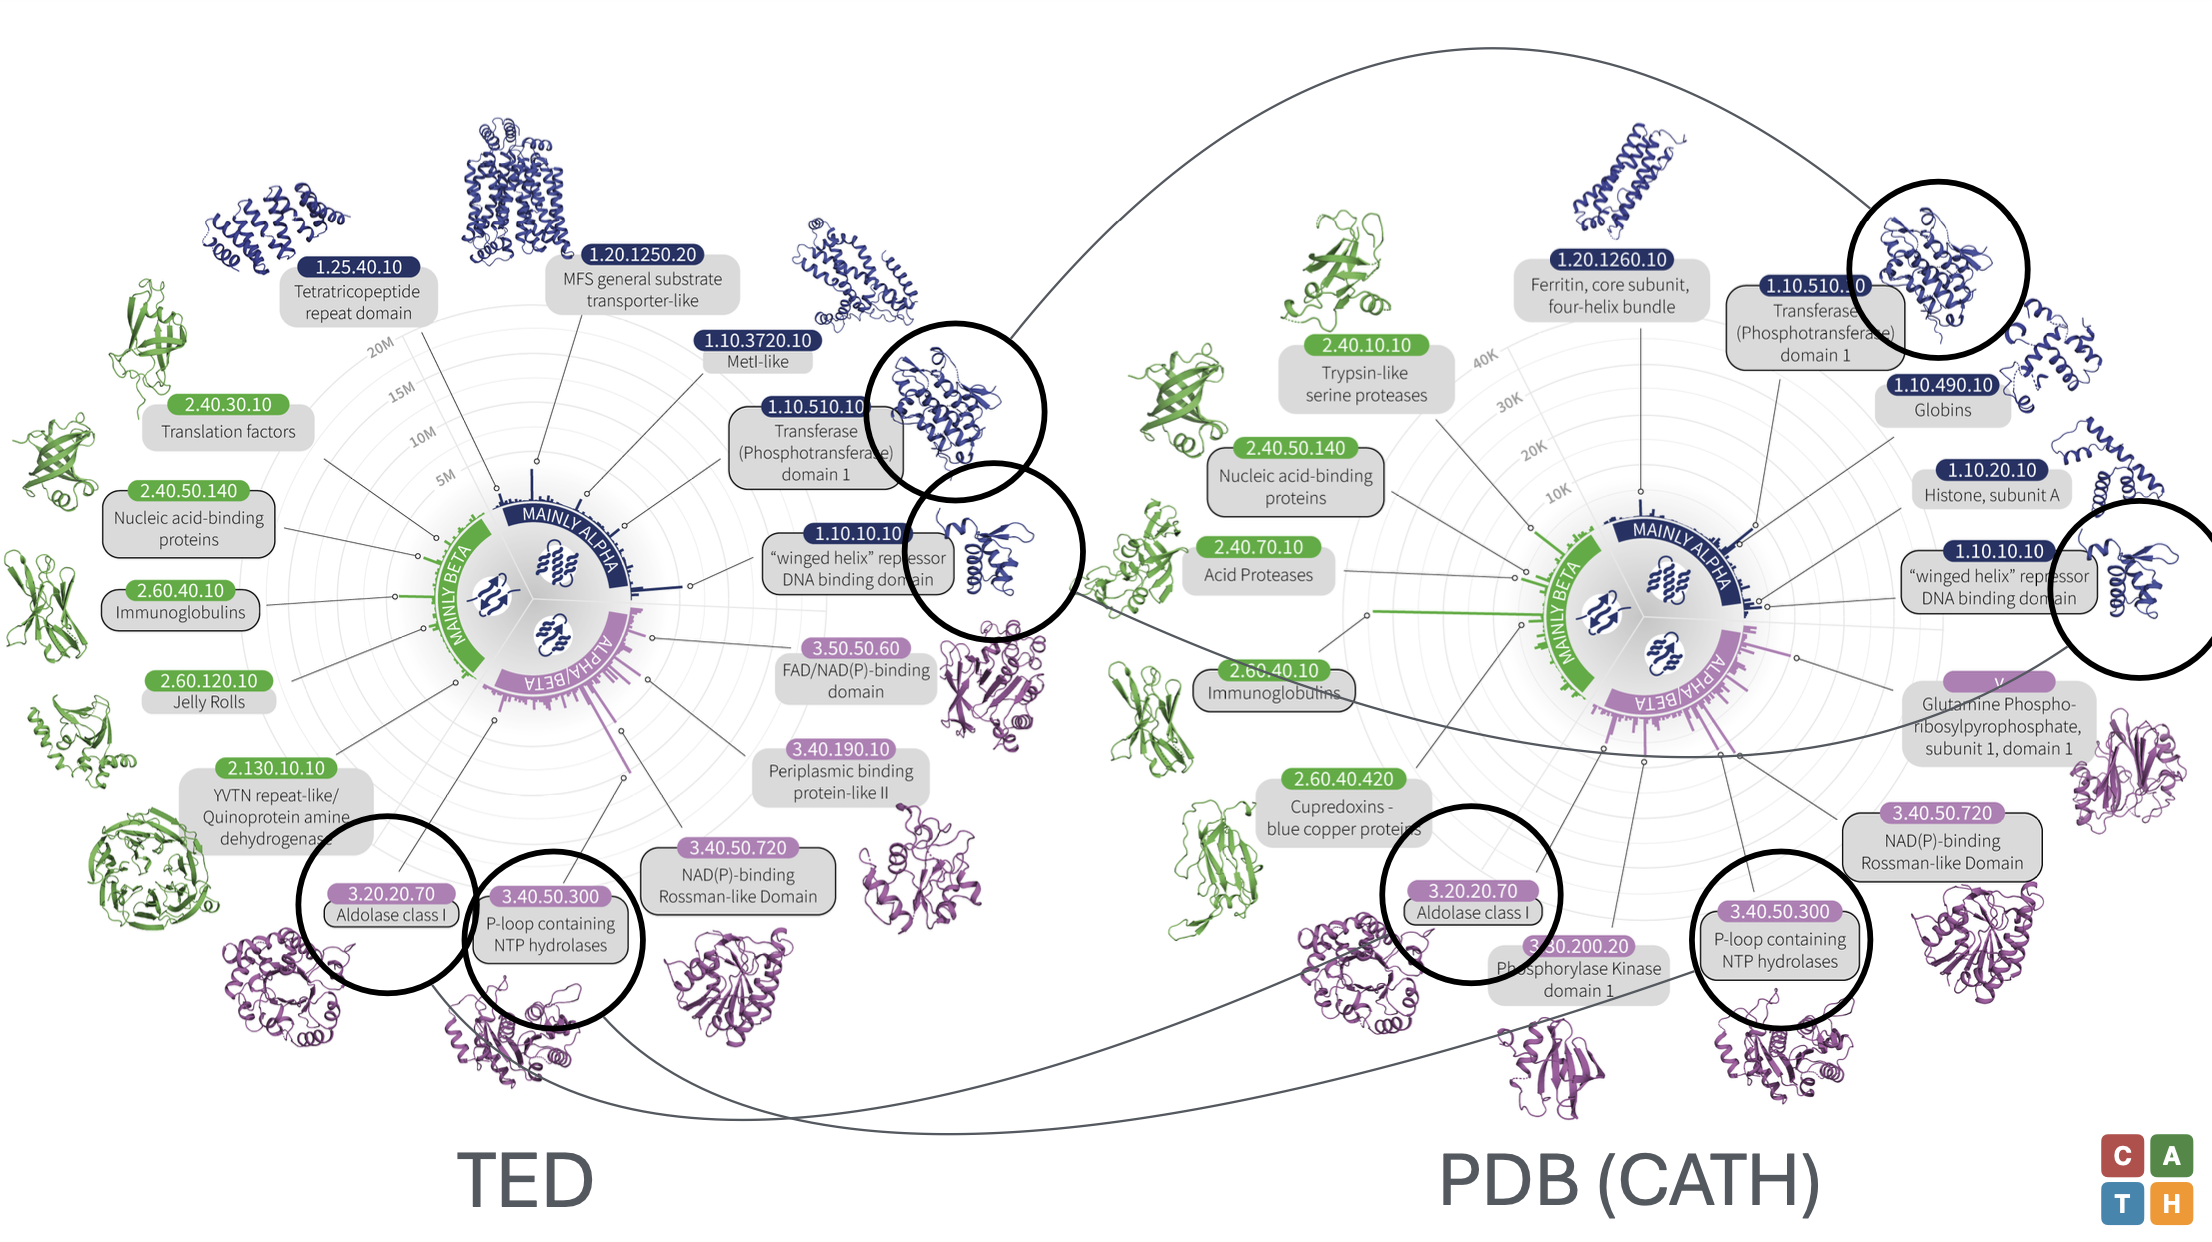
\includegraphics[width=\linewidth]{figures/ch05_cath_wheel.png}
  \caption{Comparison of CATH superfamily populations in TED (left) and PDB (right).}
  \label{fig:cath-wheel}
\end{figure*}

The difference in philosophy between SCOP and CATH is worth spelling out. SCOP
privileges evolutionary reasoning; a human expert asks ``did these proteins
descend from a common ancestor?'' and assigns accordingly. CATH privileges
reproducibility and throughput; automated algorithms do most of the work, and
human curation intervenes only at difficult boundaries. The two databases agree on
most assignments but disagree on enough cases---a non-negligible fraction of domain
superfamilies~\cite{sillitoe2021}---to remind us that protein classification is
partly a matter of convention.


\section{Measuring structural similarity}
\label{sec:structural_similarity}

\begin{figure}
  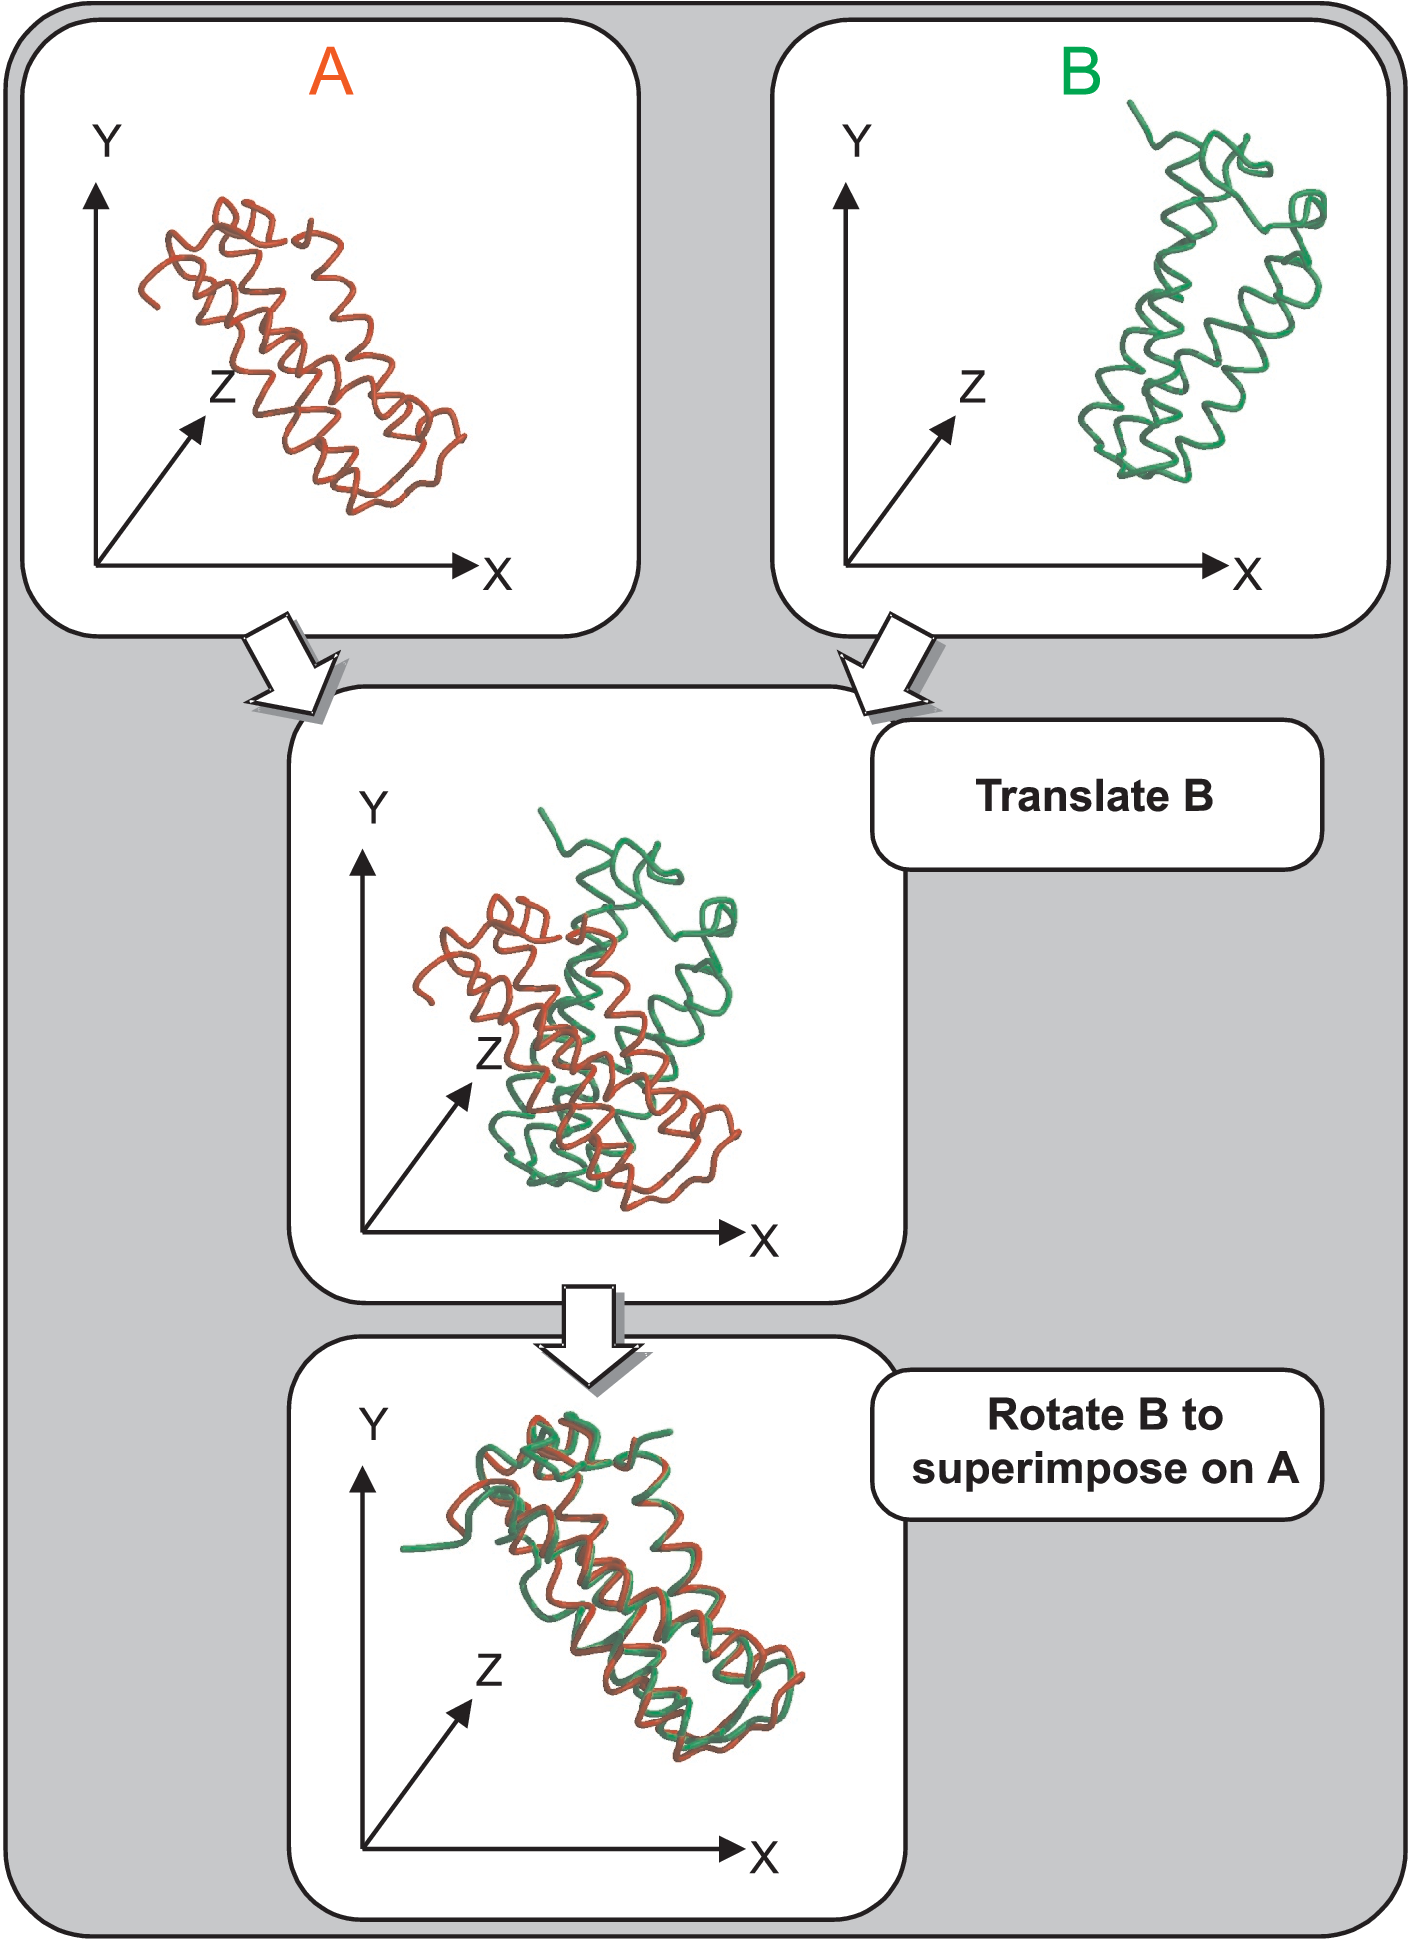
\includegraphics[width=\linewidth]{figures/ch05_structural_alignment.png}
  \caption{Structural superposition by translation and rotation.}
  \label{fig:structural-alignment}
\end{figure}

\newthought{Any classification scheme} must rest on a quantitative measure of how
alike two structures are. The most obvious measure is the root-mean-square
deviation (RMSD) of atomic positions after optimal superposition. Given two sets of
$n$ corresponding atoms with positions $\{\vx_i\}$ and $\{\bm{y}_i\}$, the
optimal rotation $\mR$ and translation $\vt$ minimize
\begin{equation}
\label{eq:rmsd-fold-space}
\text{RMSD} = \sqrt{\frac{1}{n}\sum_{i=1}^{n} \|\mR\vx_i + \vt - \bm{y}_i\|^2}.
\end{equation}
Kabsch showed in 1976 that the optimal rotation can be found in closed form from
the singular value decomposition of the cross-covariance matrix of the two
coordinate sets~\cite{kabsch1976}.\sidenote{The Kabsch algorithm computes the $3\times 3$ matrix
$H = \sum_i (\vx_i - \bar{\vx})(\bm{y}_i - \bar{\bm{y}})^\top$, takes its SVD
$H = U\Sigma V^\top$, and returns $\mR = V \diag(1,1,\det(VU^\top)) U^\top$.
The determinant correction ensures a proper rotation rather than a
reflection.}

RMSD has two serious problems. First, it depends on the length of the alignment.
Comparing a 50-residue domain to another 50-residue domain might give an RMSD of
1.5~\AA, which is excellent; comparing two 300-residue proteins might also give
1.5~\AA, which is extraordinary. The same number means different things at
different lengths. Second, RMSD is sensitive to outliers. A single misaligned loop
of ten residues displaced by 15~\AA\ can inflate the overall RMSD from 2~\AA\ to
4~\AA, even though the structural cores superimpose well.

\newthought{The TM-score}, introduced by Zhang and Skolnick in
2004~\cite{zhang2005}, was designed to address both problems. It is defined as
\begin{equation}
\label{eq:tmscore}
\text{TM-score} = \frac{1}{L}\sum_{i=1}^{L_{\text{ali}}}
  \frac{1}{1 + \left(\dfrac{d_i}{d_0(L)}\right)^2},
\end{equation}
where $L$ is the length of the target protein, $L_{\text{ali}}$ is the number of
aligned residues, $d_i$ is the distance between the $i$-th pair of aligned
residues after superposition, and
\begin{equation}
\label{eq:d0}
d_0(L) = 1.24\,\sqrt[3]{L - 15} - 1.8
\end{equation}
is a length-dependent distance scale.\sidenote{The constants 1.24, 15, and 1.8
were chosen empirically so that the average TM-score of two randomly related
proteins of any length is approximately 0.17.} The Lorentzian form
$1/(1+(d_i/d_0)^2)$ gives full weight to well-aligned residue pairs (those with
$d_i \ll d_0$) and negligible weight to pairs far apart. This makes TM-score
insensitive to local structural deviations in poorly aligned regions, directly
solving the outlier problem of RMSD.

TM-score lies in the interval $(0, 1]$, and because $d_0$ grows with $L$, the
score is length-independent: a pair of 80-residue proteins and a pair of
400-residue proteins with the same global fold will receive similar TM-scores.
Empirically, TM-score $> 0.5$ indicates that two proteins share the same fold
with high confidence. Below 0.3, proteins are almost certainly unrelated. The
region between 0.3 and 0.5 is ambiguous, which is appropriate: fold space does
not have sharp boundaries.


\section{Structure alignment algorithms}
\label{sec:alignment_algorithms}

\newthought{Computing TM-score requires} a structural alignment: a correspondence
between residues in two proteins, together with the superposition that minimizes
the distances between matched pairs. Finding the optimal alignment is
computationally hard in general (it is an instance of the maximum-weight matching
problem in three dimensions), so practical methods use heuristic strategies.

TM-align~\cite{zhang2005} works by iterating between two steps. Given a current
alignment, it computes the optimal superposition by the Kabsch algorithm
restricted to aligned residue pairs. Given a current superposition, it computes a
new alignment by dynamic programming, using a scoring function derived from the
TM-score formula. The procedure alternates until convergence, typically in three
to five iterations. Multiple initial alignments seeded from secondary-structure
matching or gapless threading ensure that the algorithm does not get stuck in a
poor local optimum. TM-align runs in time roughly proportional to $L^2$ and
finishes in seconds even for large proteins.

\newthought{SSAP} (Sequential Structure Alignment Program), developed by Christine
Orengo and colleagues for use in CATH, takes a different approach. Rather than
comparing atomic coordinates directly, SSAP represents each residue by a vector of
intramolecular distances to all other residues in the protein. Two proteins are
compared by aligning these distance vectors using double dynamic programming: a
first pass aligns individual residue environments, and a second pass assembles
these local matches into a globally consistent alignment. SSAP scores range from 0
to 100; scores above 80 indicate the same fold, and scores above 70 suggest
structural similarity worth investigating.\sidenote{SSAP is one of the oldest
structure-comparison methods still in active use. Its double-dynamic-programming
approach predates distance-matrix methods like Dali and coordinate-based methods
like TM-align.}

\newthought{Dali}, developed by Liisa Holm in the early 1990s~\cite{holm1993}, compares proteinscompares proteins
by their intramolecular distance matrices. Each protein is reduced to an
$n \times n$ matrix $D$ where $D_{ij}$ is the distance between the $C_\alpha$
atoms of residues $i$ and $j$. Two proteins are compared by finding the alignment
that maximizes the similarity between submatrices of their respective distance
matrices. The similarity is measured by a score that emphasizes contacts (short
distances) and downweights long-range pairs. Dali uses a Monte Carlo optimization
to search the space of possible alignments, making it slower than TM-align but
sometimes more sensitive for detecting remote structural similarities. The FSSP
database (Fold classification based on Structure-Structure alignment of Proteins)
was built entirely from all-against-all Dali comparisons of the PDB.

Each of these algorithms has a regime where it performs best. TM-align is fast and
gives a clean, interpretable score; it is the current standard for large-scale
comparisons and benchmarking. SSAP captures local structural detail well and
remains integral to the CATH pipeline. Dali excels at detecting distant
relationships where the overall fold is similar but local deviations are large.
In practice, large classification projects use multiple methods and reconcile
disagreements manually or by majority vote.


\section{Structural domains}
\label{sec:domains}

\begin{marginfigure}
  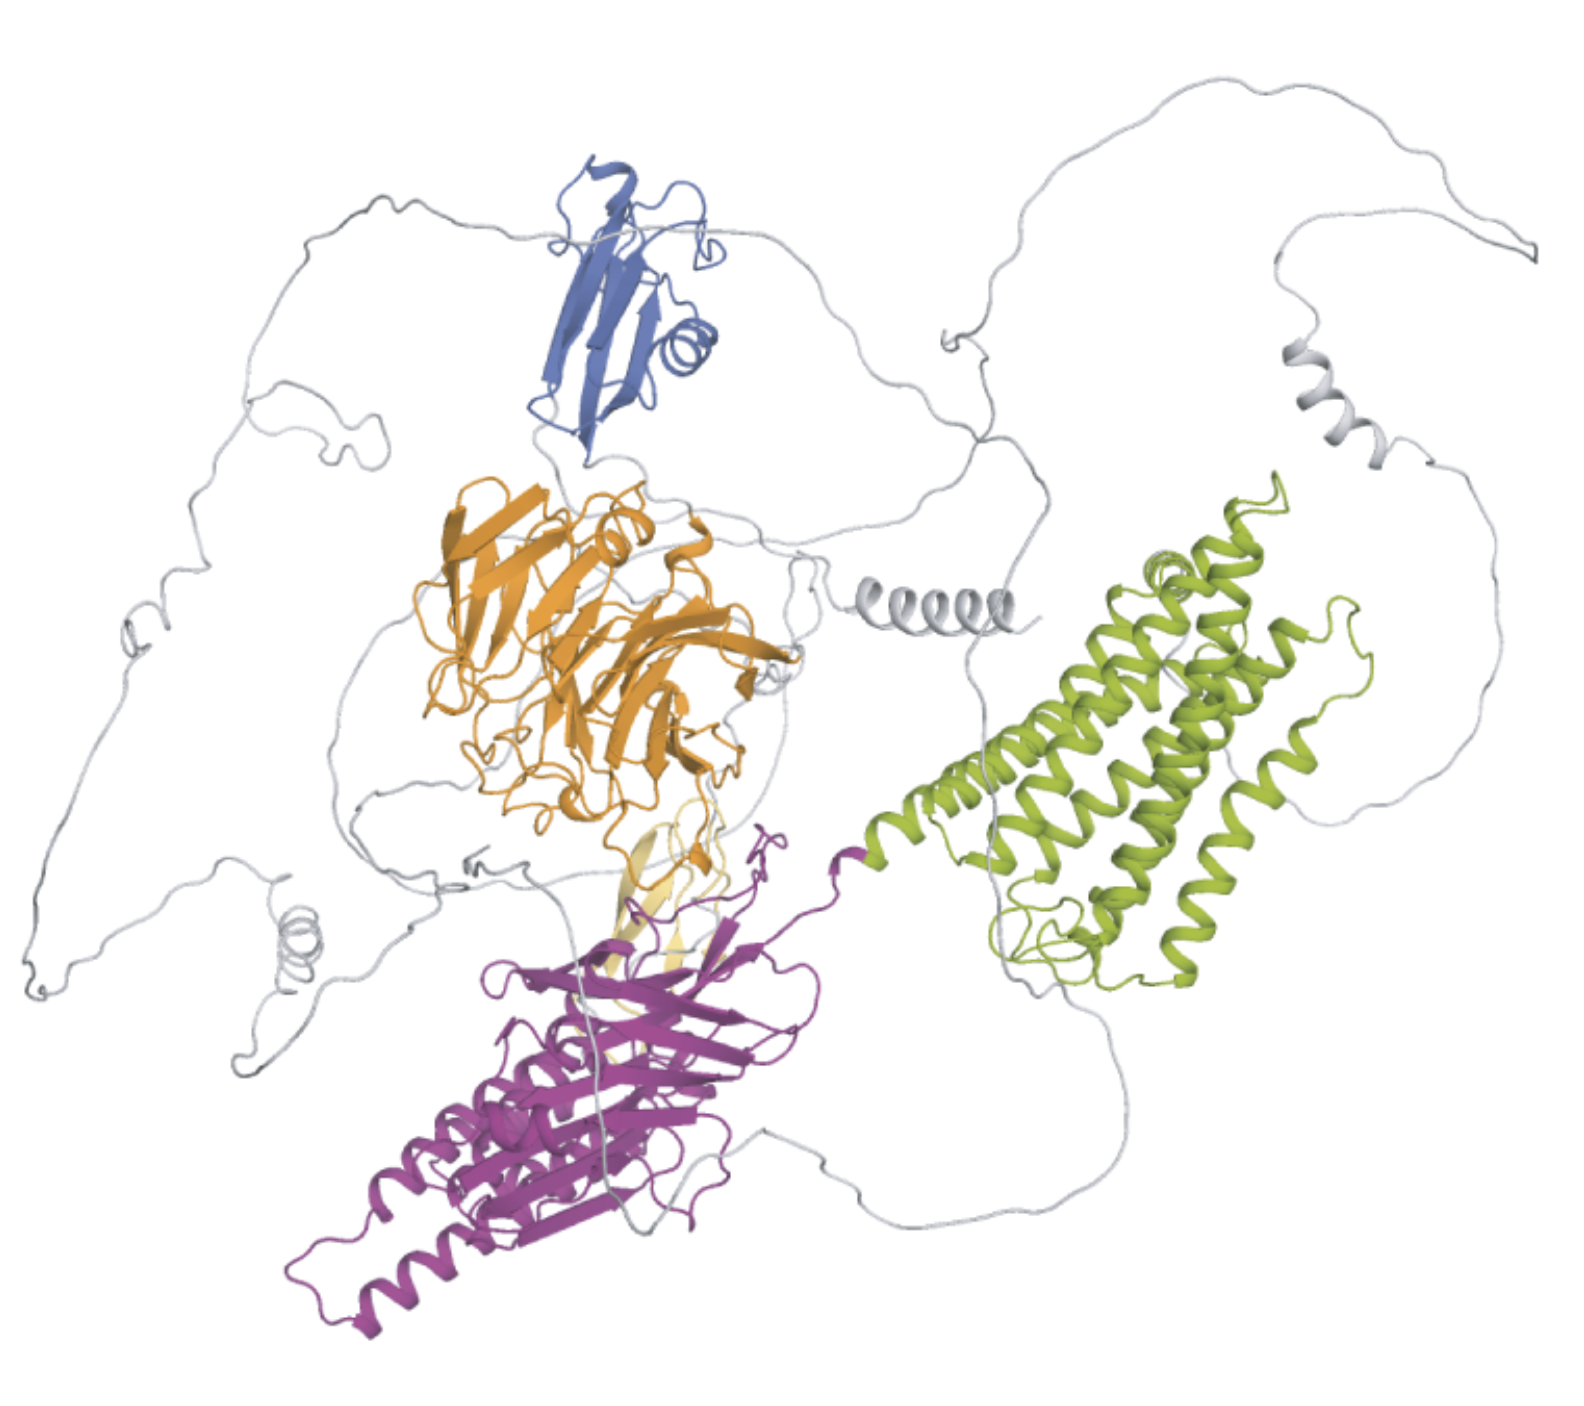
\includegraphics[width=\linewidth]{figures/ch05_multidomain_protein.png}
  \caption{A multi-domain protein with four domains shown in distinct colors.}
  \label{fig:multidomain-protein}
\end{marginfigure}

\newthought{Most proteins longer} than about 200 residues fold into two or more
distinct structural domains. A domain is a compact, semi-independent region of the
polypeptide chain that folds into a stable three-dimensional structure and often
functions as an evolutionary unit, appearing in different combinations across
different proteins. Domain boundaries rarely split secondary-structure elements;
they usually fall in loops connecting elements that contact each other within the
domain but not across domains.

Classification operates at the domain level, not the chain level. A protein with
three domains may have each domain assigned to a different fold in SCOP or
topology in CATH. This is sensible from both structural and evolutionary
perspectives: gene duplication, fusion, and recombination shuffle domains more
frequently than they create entirely new folds. But it means that any
classification pipeline must begin by parsing multi-domain proteins into their
constituent domains, and this parsing step is itself nontrivial.

Manual domain assignment (as in early SCOP) uses visual inspection and expert
knowledge of protein families. Automated methods attack the problem
computationally. PDP (Protein Domain Parser) identifies domains by analyzing the
contact map~\cite{alexandrov2003}: it looks for clusters of residues that are in close spatial contact
with each other but not with residues in other clusters. The algorithm recursively
splits the chain at the boundary that minimizes inter-domain contacts. SWORD
(Swift and Optimized Recognition of Domains) uses a similar principle but
incorporates secondary-structure information and is optimized for speed on the
scale of the entire PDB~\cite{postic2017}.\sidenote{Domain boundaries predicted by automated methods
agree with expert assignments roughly 80--85\% of the time. The remaining cases
tend to be discontinuous domains, where the chain leaves one domain, contributes a
segment to another, and returns.}

\newthought{Gene3D extends} domain classification to the genome scale~\cite{lees2012gene3d}. Starting
from CATH superfamily assignments for experimentally determined structures,
Gene3D builds hidden Markov models for each superfamily and scans genomic
sequences against these models. A match implies that the query sequence will fold
into a structure assignable to that CATH superfamily. The result is a mapping from
every gene in hundreds of sequenced genomes to its predicted domain architecture.
This mapping connects structural classification (defined on 3D coordinates) to
sequence annotation (defined on amino acid strings), creating a bridge between the
two worlds.


\section{Integrative classification with InterPro}
\label{sec:interpro}

\newthought{No single classification} system captures all aspects of protein
function and evolution. Pfam provides sequence-based family definitions using
profile HMMs trained on multiple sequence alignments. Gene3D provides
structure-based superfamily assignments projected onto genomes. SUPERFAMILY does
something similar using SCOP superfamilies as the reference. PROSITE defines
short sequence patterns and profiles that identify functional sites, active-site
residues, and binding motifs. Each database sees the protein universe from a
different angle, and each misses relationships that others capture.

InterPro integrates these resources into a unified classification~\cite{blum2021}. For each
protein, InterPro collects the annotations assigned by Pfam, Gene3D,
SUPERFAMILY, PROSITE, PANTHER, CDD, and a dozen other member databases, resolves
overlaps and conflicts, and produces a consensus domain annotation. A protein
annotated as ``Rossmann fold, NAD-binding superfamily'' by Gene3D and matched to
the ``short-chain dehydrogenase'' family by Pfam receives a merged InterPro entry
that records both relationships and links them. The system is updated with each
UniProt release, ensuring that newly sequenced proteins receive classification
within weeks of deposition.

The value of integration is not just convenience. Different member databases use
different algorithmic approaches and different evolutionary hypotheses. When they
agree, confidence is high. When they disagree, the disagreement flags a protein
that deserves closer inspection. InterPro makes these agreements and disagreements
explicit, which is more honest than presenting any single classification as
definitive.


\section{Classification in the AlphaFold era}
\label{sec:alphafold_era}

\newthought{The AlphaFold Protein Structure Database}, released in 2021 and
expanded in 2022, contains predicted structures for over 200 million protein
sequences. This changed the classification problem qualitatively. When the PDB
held two hundred thousand experimental structures, classification was already
challenging but computationally manageable. With two hundred million predicted
structures, even fast algorithms like TM-align become expensive if applied
naively in all-against-all mode.

\begin{figure*}
  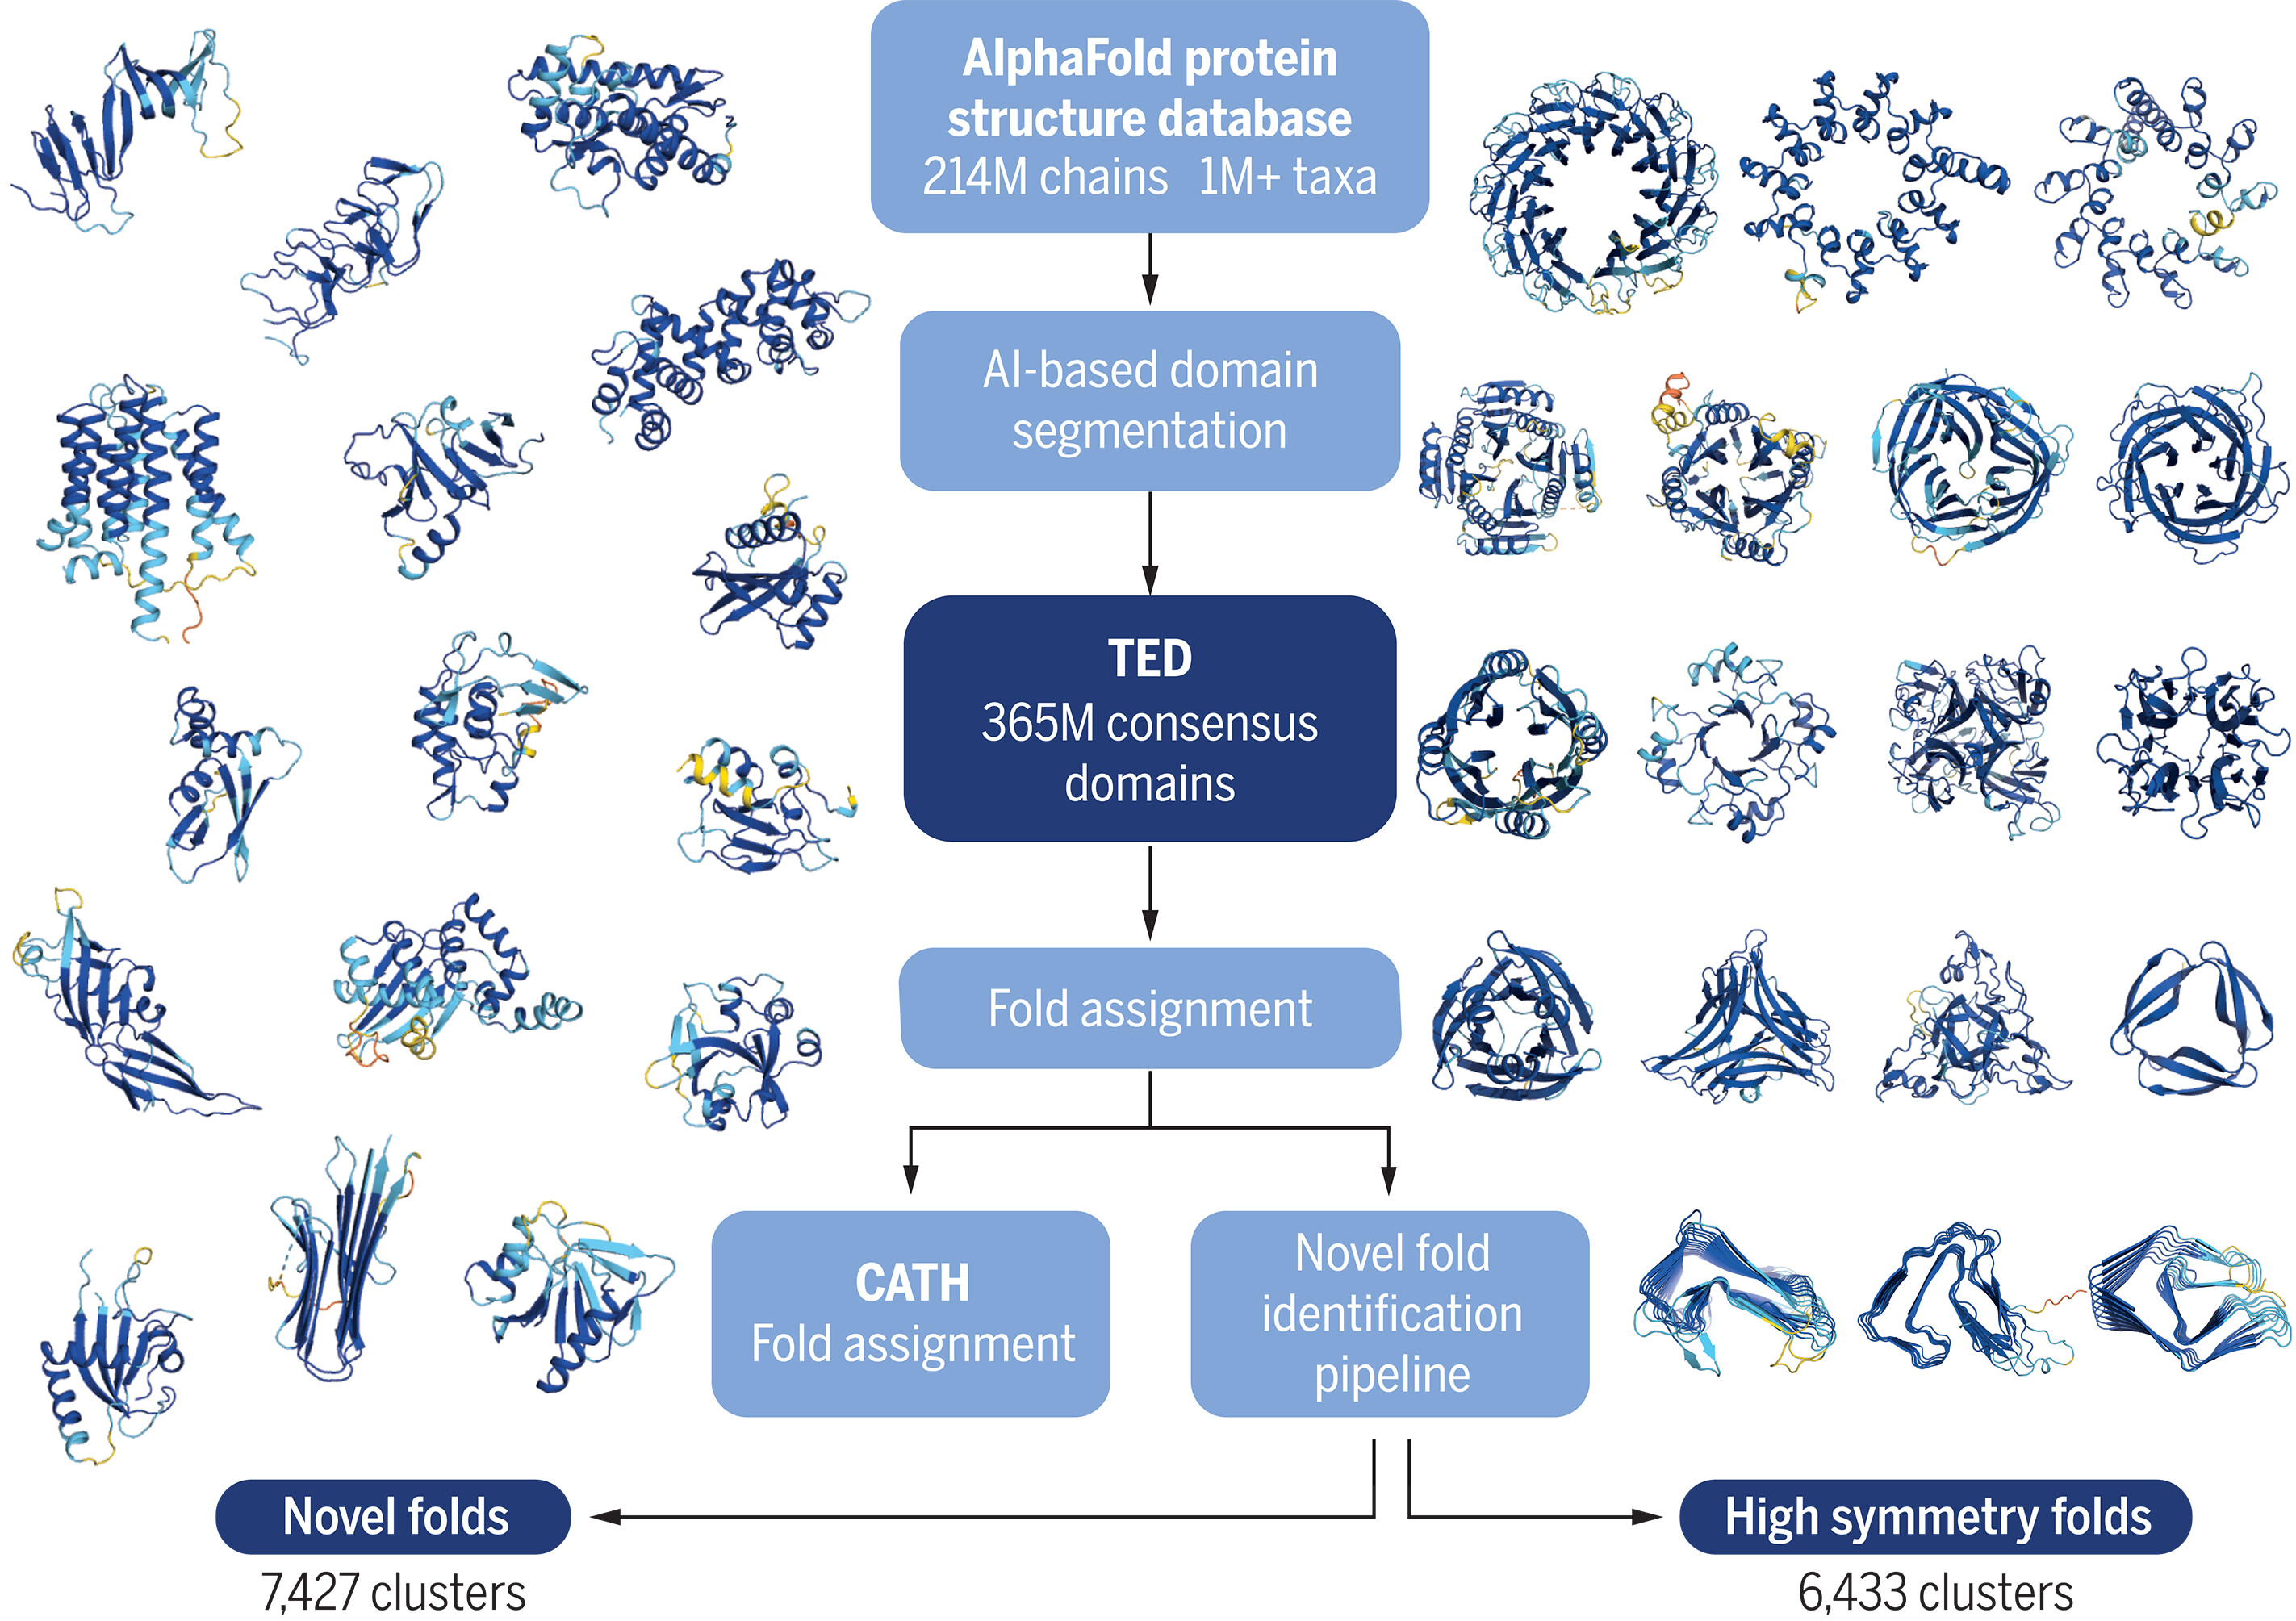
\includegraphics[width=\linewidth]{figures/ch05_ted_pipeline.jpeg}
  \caption{The TED pipeline: from AlphaFold database to domain segmentation, fold assignment, and novel fold identification.}
  \label{fig:ted-pipeline}
\end{figure*}

The Encyclopedia of Domains (TED), developed by the Orengo group at UCL, addresses
this challenge~\cite{lau2024ted}. TED takes AlphaFold-predicted structures, parses them into domains
using automated boundary-detection methods, and assigns each domain to a CATH
superfamily by structure comparison. Domains that cannot be matched to any known
superfamily are clustered among themselves to identify potentially novel folds. The
project found that the vast majority of AlphaFold-predicted domains belong to
known CATH superfamilies, but several thousand clusters represent structural
topologies not observed in the experimental PDB. Whether these are genuinely novel
folds or artifacts of prediction errors is an open question that requires
experimental validation.\sidenote{Preliminary analysis of TED clusters suggests
that many ``novel'' folds come from dark proteomes: organisms or protein families
that have received little experimental attention. Some of these predictions have
since been confirmed by cryo-EM structures.}

The availability of predicted structures also forces a rethinking of what
classification means. SCOP and CATH were built on experimental structures, where
the coordinates are known to a resolution of 1--3~\AA\ and domain boundaries can
be validated against electron density or diffraction data. AlphaFold predictions
come with per-residue confidence scores (pLDDT), and low-confidence regions may
correspond to disorder rather than a defined fold. A classification system that
ingests predicted structures must account for confidence, treating high-pLDDT
domains differently from low-pLDDT segments that may not adopt a stable
tertiary structure at all.


\section{The structure of fold space}
\label{sec:fold_space}

\newthought{Is the space of protein folds} continuous or discrete? The question
has no clean answer, and the answer depends on the resolution at which one looks.
At the level of SCOP folds or CATH topologies, the number of distinct folds
observed in nature appears to be limited: roughly 1,500 in SCOP, roughly 1,400
topologies in CATH, with the rate of discovery of genuinely new folds slowing each
year. This suggests that evolution has explored a finite (though large) set of
structural solutions, constrained by the physics of chain packing and the
kinetics of folding.

But between any two folds, one can often find intermediate structures that blur
the boundary. The $\beta$-barrel family, for instance, includes barrels with 6, 8,
10, 12, 14, and 16 strands, with varying shear numbers and strand tilts. Is a
16-stranded barrel the ``same fold'' as an 8-stranded barrel? SCOP says no; the
topology is different. But the barrels form a continuum parameterized by strand
number and shear, and any threshold for ``same'' versus ``different'' is
arbitrary.\sidenote{Kolodny and colleagues showed that if one embeds SCOP
domains in a high-dimensional space using pairwise structural-similarity scores,
the resulting cloud of points does not form well-separated clusters~\cite{kolodny2005}. Fold space
looks more like a continuous manifold with regions of higher density than like a
set of discrete islands.}

This observation does not invalidate classification. Maps are useful even when
the territory is continuous. But it should temper any expectation that there
exists a single ``correct'' classification of protein structures. SCOP, CATH, and
other systems are different maps of the same territory, drawn with different
projections and for different purposes.


\section{Chapter notes}
\label{sec:ch5_notes}

The SCOP database was described by Murzin, Brenner, Hubbard, and Chothia in 1995~\cite{murzin1995}.
The most commonly cited version is SCOP 1.75, the last release curated in the
original framework. SCOP2, which adopts a directed acyclic graph rather than a
tree, was described by Andreeva et al.\ \cite{andreeva2014}. CATH was introduced by Orengo et al.\ in
1997~\cite{orengo1997} and has been updated continuously; the current version
(CATH-Gene3D 4.3) classifies over 500,000 domains. Both databases are freely
available and regularly used as gold standards for benchmarking structure-comparison
methods.

The TM-score and TM-align algorithm were introduced together by Zhang and
Skolnick~\cite{zhang2005}. The 0.5 threshold for fold similarity was validated
empirically against SCOP classifications by Xu and Zhang~\cite{xu2010tm}, who showed that
TM-score discriminates same-fold from different-fold pairs with an accuracy
exceeding 95\%. A later analysis by Murzin noted cases where TM-score disagrees
with SCOP assignments, particularly for long proteins with multiple domains; these
cases highlight the dependence of all similarity metrics on the choice of which
residues to include in the comparison.

The Kabsch algorithm for optimal superposition was published in 1976~\cite{kabsch1976} and remains
the standard method. Equivalent formulations using quaternions~\cite{horn1987} or
eigenvalue decomposition (by Diamond, 1988) exist; all produce identical results
and differ only in implementation details. For the singular cases where the SVD
solution is ambiguous (when the cross-covariance matrix is degenerate), the
determinant correction shown in the sidenote ensures a proper rotation.

Dali was introduced by Holm and Sander~\cite{holm1993}. The original FSSP database is no
longer actively maintained, but the Dali server continues to provide on-the-fly
structure comparisons and is widely used for finding structural neighbors of a
newly determined structure. SSAP was first described by Taylor and Orengo~\cite{taylor1990}
and refined in subsequent papers; its integration into the CATH pipeline is
described in the 1997 CATH paper.

InterPro, first described by Mulder et al.~\cite{mulder2003} and surveyed in recent releases~\cite{blum2021}, is maintained by the European
Bioinformatics Institute and updated with each UniProt release. As of 2024, it
integrates 14 member databases and provides annotations for over 47 million
distinct protein sequences.

The Encyclopedia of Domains (TED) is described by Lau et al.~\cite{lau2024ted}.
Its finding that AlphaFold predictions contain thousands of potentially novel
folds has stimulated experimental work aimed at validating these predictions, with
early results from cryo-EM confirming several previously unobserved topologies.
The question of how classification should handle predicted structures with varying
confidence remains an active area of methodological development.

For a broader perspective on the geometry of fold space, see the work of Kolodny,
Koehl, and Levitt~\cite{kolodny2005}, who mapped SCOP domains into a continuous
high-dimensional space and found evidence against a purely discrete view of folds.
Taylor (2007) offered a different perspective, arguing that fold space has a
fractal character: self-similar at multiple scales but not truly continuous.
Whether one finds protein folds to be discrete or continuous depends, in the end,
on the similarity threshold one chooses, which is another way of saying that the
answer depends on the question being asked.
